%%%%%%%%%%%%%%%%%%%%%%%%%%%%%%%%%%%%%%%%%%%%%%%%%%%%%%%%%%%%%
% ECE 445 SENIOR DESIGN TEMPLATE
%%%%%%%%%%%%%%%%%%%%%%%%%%%%%%%%%%%%%%%%%%%%%%%%%%%%%%%%%%%%%
\documentclass[letterpaper,10pt]{article}

%%%%%%%%%%%%%%%%%%%%%%%%%%%%%%%%%%%%%%%%%%%%%%%%%%%%%%%%%%%%%
% The preamble starts here.
% You can add other packages that you want to use by using
% \usepackage command in the preamble.
% However, DO NOT change the settings that are already placed
% below unless you really know what you are doing.
%%%%%%%%%%%%%%%%%%%%%%%%%%%%%%%%%%%%%%%%%%%%%%%%%%%%%%%%%%%%%

% some commonly used packages
\usepackage{graphicx}
\usepackage{color,soul}
\usepackage{amsmath}
\usepackage{amsthm}
\usepackage{amsfonts}
\usepackage{setspace}
\usepackage{longtable}
\usepackage{url}
\usepackage{float}
\usepackage{caption}
\usepackage[colorlinks=true,linkcolor=black,citecolor=black]{hyperref}
\usepackage[top=1in, bottom=1in, left=1in, right=1in]{geometry}% set the page margins to 1 inch

% use the fancyhdr package to maintain the format of the page numbers,
% which is useful when the text color is changed
\usepackage{fancyhdr}
\fancyhf{}
\renewcommand{\headrulewidth}{1pt}
\renewcommand{\footrulewidth}{0pt}
\fancyfoot[C]{\textcolor{black}{\thepage}}
\fancyhead[L]{
\includegraphics[width=2cm]{University-of-Illinois-logo.jpg}}
\fancyhead[R]{\small{Infantry I.F.F. Mock Design Review - Meyers \& Prince}}

% paralist provides extended list environments
\usepackage{paralist}
\setlength{\plitemsep}{0pt}

% define the color for section and subsection titles
\usepackage{xcolor}
\definecolor{titlecolor}{RGB}{31,73,125}
\definecolor{subtitlecolor}{RGB}{79,129,189}

% change the style of the section and subsection titles
\usepackage{titlesec}
\titleformat{\section}{\color{titlecolor}\Large\bf}{\color{titlecolor}\thesection}{0.8em}{}
\titleformat{\subsection}{\color{subtitlecolor}\large\bf}{\color{subtitlecolor}\thesubsection}{1em}{}
\titleformat{\subsubsection}{\color{subtitlecolor}\normalsize\bf}{\color{subtitlecolor}\thesubsubsection}{1.2em}{}
\titlespacing{\section}{0pt}{0em}{0em}
\titlespacing{\subsection}{0pt}{0em}{0em}
\titlespacing{\subsubsection}{0pt}{0em}{0em}

% change the style of the table of contents
\usepackage{titletoc}
\titlecontents{section}[1.5em]{}{\contentslabel{1.5em}}{\hspace*{-1.5em}}{\titlerule*[0.5pc]{.}\contentspage}
\titlecontents{subsection}[3em]{}{\contentslabel{2.1em}}{\hspace*{-2.1em}}{\titlerule*[0.5pc]{.}\contentspage}
\titlecontents{subsubsection}[5.1em]{}{\contentslabel{2.7em}}{\hspace*{-2.7em}}{\titlerule*[0.5pc]{.}\contentspage}

% command for centering texts in a fixed width table cell
\newcommand{\centpcol}{\leftskip\fill \rightskip\fill}

% command for setting the style of the appendix titles
\newcommand{\setappenstyle}{
	\titleformat{\section}{\color{titlecolor}\Large\bf}{\color{titlecolor}Appendix \Alph{section}}{0.8em}{}
	\titlecontents{section}[0em]{}{Appendix \thecontentslabel \hspace{1em}}{}{\titlerule*[0.5pc]{.}\contentspage}
}

% define the style of the title of the paper
\newcommand{\thetitle}[1]{\title{\begin{huge}{\bf #1}\end{huge} \color{subtitlecolor}\rule[25pt]{\textwidth}{1pt}}}

% define the style of the author
\newcommand{\theauthor}[3]{
	\author{\vspace{.4in}\\
	\textcolor{black}{By}\\
	#1
	\vspace{1in}\\
	\textcolor{black}{ECE 445 Mock Design Review -} #2\\
	\textcolor{black}{TA:} #3
	\vspace{1in}}
}

% define the style of figure's caption
\newcommand{\figcap}[1]{
	\captionsetup{format=plain,font={small,color=subtitlecolor,singlespacing},margin={0pt,0pt}}
	\caption{\textcolor{subtitlecolor}{#1}}
	\vspace{-5pt}
}

% define the style of table's caption
\newcommand{\tablecap}[1]{
	\captionsetup{format=plain,font={bf,normalsize,singlespacing,color=black},margin={0pt,0pt}}
	\caption{\textcolor{black}{#1}}
	\vspace{-5pt}
}


\newcommand{\buildtoc}{
	\clearpage
	\singlespacing
	\tableofcontents
	\onehalfspacing
}

% set indentations and the space between paragraghs
\setlength{\parindent}{0pt}
\setlength{\parskip}{8pt}

%%%%%%%%%%%%%%%%%%%%%%%%%%%%%%%%%%%%%%%%%%%%%%%%%%%%%%%%%%%%%
% PREAMBLE ENDS HERE, DOCUMENT STARTS BELOW
%%%%%%%%%%%%%%%%%%%%%%%%%%%%%%%%%%%%%%%%%%%%%%%%%%%%%%%%%%%%%

\begin{document}

% don't change these
\pagestyle{empty}
\doublespacing

% put the title of your project here. DO NOT include the brackets.
\thetitle{{I.F.F. (Identification Friend or Foe) System}}

% put your names here. seperate by \\. DO NOT include the brackets.
\theauthor{
	{Eric Meyers (emeyer7)}\\
	{Noah Prince (nprince2)}\\
}
{ % put the semester info here. DO NOT include the brackets.
	{Spring 2016}
}
{ % put your TA's name here. DO NOT include the brackets.
	{Braedon Salz}
}

% put the date and project number here. DO NOT include the brackets.
\date{
{February 18th, 2016}\\
Project No. 11
\clearpage
}

% don't change these
\maketitle
\pagestyle{fancy}
\begin{spacing}{1.15}


% build the table of contents. 
\color{black}
\buildtoc
\pagenumbering{gobble}
\section*{Acronyms \& Pre-Requisite Information}
\begin{itemize}
	\item MCU - Microcontroller Unit
	\item R.F. - Radio Frequency
	\item T.I. - Texas Instruments
	\item PPM - Parts Per Million - used to designate accuracy of crystal oscillator 
\end{itemize}
\clearpage
\setcounter{page}{1}
\pagenumbering{arabic}

%SECTION 1 - Introduction - Eric
\section{Introduction}
This document is a "Mock Design Review" in preparation for the Design Review occuring during the week of February 29th, 2016. This will outline the preliminary design for one block of the entire system. The system the team decided upon was the Laser Transmission Subsystem on board the Friendly Interrogator Unit.

%SECTION 2 - Design - Eric
\section{Block Diagram}
\begin{figure} [H]
	\centering
	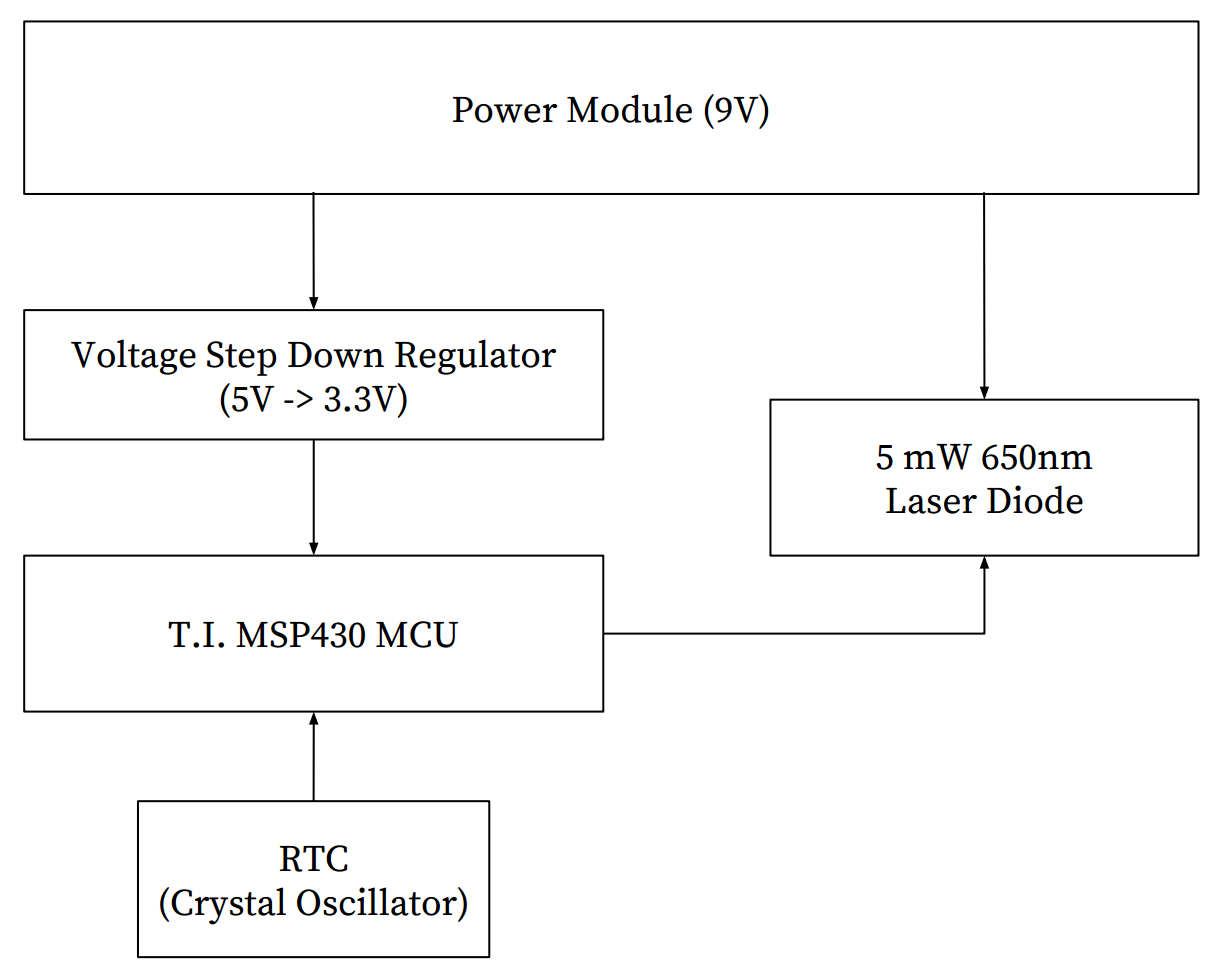
\includegraphics[scale=0.50]{Block_Diagram.png}
	\caption{Block Diagram of Laser Transmitter\label{fig:circuit-schematic}}
\end{figure}

%SECTION 5 - Block Description - Eric
\section{Block Description}
The subsystem of the Laser Transmitter will be broken down into 5 primary modules:
\begin{enumerate}
	\item Power Module
	\item Voltage Step Down Regulator
	\item Microcontroller 
	\item Real Time Clock
	\item Laser Diode
\end{enumerate}

\subsection*{Power Module}
The Power Module will consist of four standard rechargable 1.2V AA NiMH batteries. This will provide an output voltage of 4.8V when placed in series in a battery pack. Depending on the manufacture chosen and the battery model, the batteries will hold a capacity of 1000 mAh to 3000mAh. For budgetary purposes the team will choose the ladder (a battery with a smaller capacity) because this will easily satisfy the requirements of powering the module for minimum of 8 hours. The friendly interrogator unit will not be drawing much current however thre are restraints placed on the current drawn from this battery in order to satisfy the time requirement. A 1000mAh battery will supply a circuit with 125 mA for 8 hours, therefore this unit must not draw more than 125 mA, which will be achievable.

The team decided to use four standard AA 1.2V NiMH rechargable batteries instead of any other standard batteries (such as disposable AAA or AA or a 9V battery) for several reasons. For one, the laser diode (as disccussed later on) operates on a voltage from 4.5 - 5.5 voltage and this will satisfy this requirement. Also, the capacity is much higher for AA rechargable batteries than 9V batteries so therefore the team went with the obvious option of choosing the AA batteries.  

\subsection*{Voltage Step Down Regulator}
The LD1117V33 Voltage Step-Down Regulator\textsuperscript{\cite{LD1117-Voltage-Regulator}} will take the 4.8V supply input and step it down to 3.3V to supply the MSP430 MCU. The voltage regulator will supply a maximum of 900 mA of current which will be significantly less than this circuit draws.

\subsection*{Microcontroller}
This design choice was by far the most difficult. The team chose to work with an T.I. MSP430F2274 Microcontroller Unit \textsuperscript{\cite{MSP430F2274}} due to its compiler simplicity, its availability in the ECE445 Senior Design Labs (inventory) and the number of GPIO Pins on board (compared to other options, this model had several I/O pins and was the most inexpensive). Compared to many other MCUs on the market, the MSP430 is relatively well documented and there exist several support forums on the internet to assist the team throughtout the duration of the project.

\subsection*{Real Time Clock}
The Real Time Clock is not entirely neccessary for the operation of the Laser Transmitter Subsystem, however it will be neccessary for the operation of the R.F. Receiver and thus must be included in the MCU circuit. It will operate using a 32.768 kHz Crystal Oscillator (as reccomended by T.I. \textsuperscript{\cite{RTC-Implementation}}) with an accuracy of +/- 20 PPM (deviates between 32.7673 kHz and 32.7687 kHz).

\subsection*{Laser Diode}
The 5mW laser diode will operate on 3.3V at 25mA so a 1.3k$\Omega$ resistor is neccessary to drop the current being supplied to the diode down to this threshold. This laser diode will prode a beam width of \_\_\_

Due to safety and ethical considerations, the requirements have changed for the divergence of the beam. The proposal stated a requirement of a 5-6 ft diameter beam at 50, 150, and 300 m (with optical adjustments allowed). 

With some tolerance, the PIN photodiode can register an irradiance of 9 $\frac{W}{m^2}$. The laser required to achieve this irradiance is a function of the laser power and the radius of the beam. With relatively short distances of 0-300 m, atmospheric deflection of light is negligible. 

Using trigonometry, the power as a function of radius is given by $P = \pi r^2  E_{req} $, where $r$ is the radius (in meters) and $E_{req}$ is the required irradiance of 9 $\frac{W}{m^2}$. 

For a diameter equal to the one stated in the proposal ($\approx 1.6764 m$), a $\pi (0.8382)^2(9) \approx 20 mW$ laser is needed. A $20 mW$ laser is a Class 3B laser, and is considered dangerous. For the scope of this senior design project, a $5mW$ laser will be used instead. 

The radius achieved using a $5 mW$ laser is given by $\sqrt{\frac{P}{E_{req} \pi}} = 0.420522 m$. This is approximately a $2.75 ft$ diameter beam, which is still the size of a person's chest. 


%SECTION 3 - Circuit Schematic - Eric
\section{Circuit Schematic}
The circuit schematic is for the Laser Transmission Subsystem on the Friendly Interrogator Unit.
\begin{figure} [H]
	\centering
	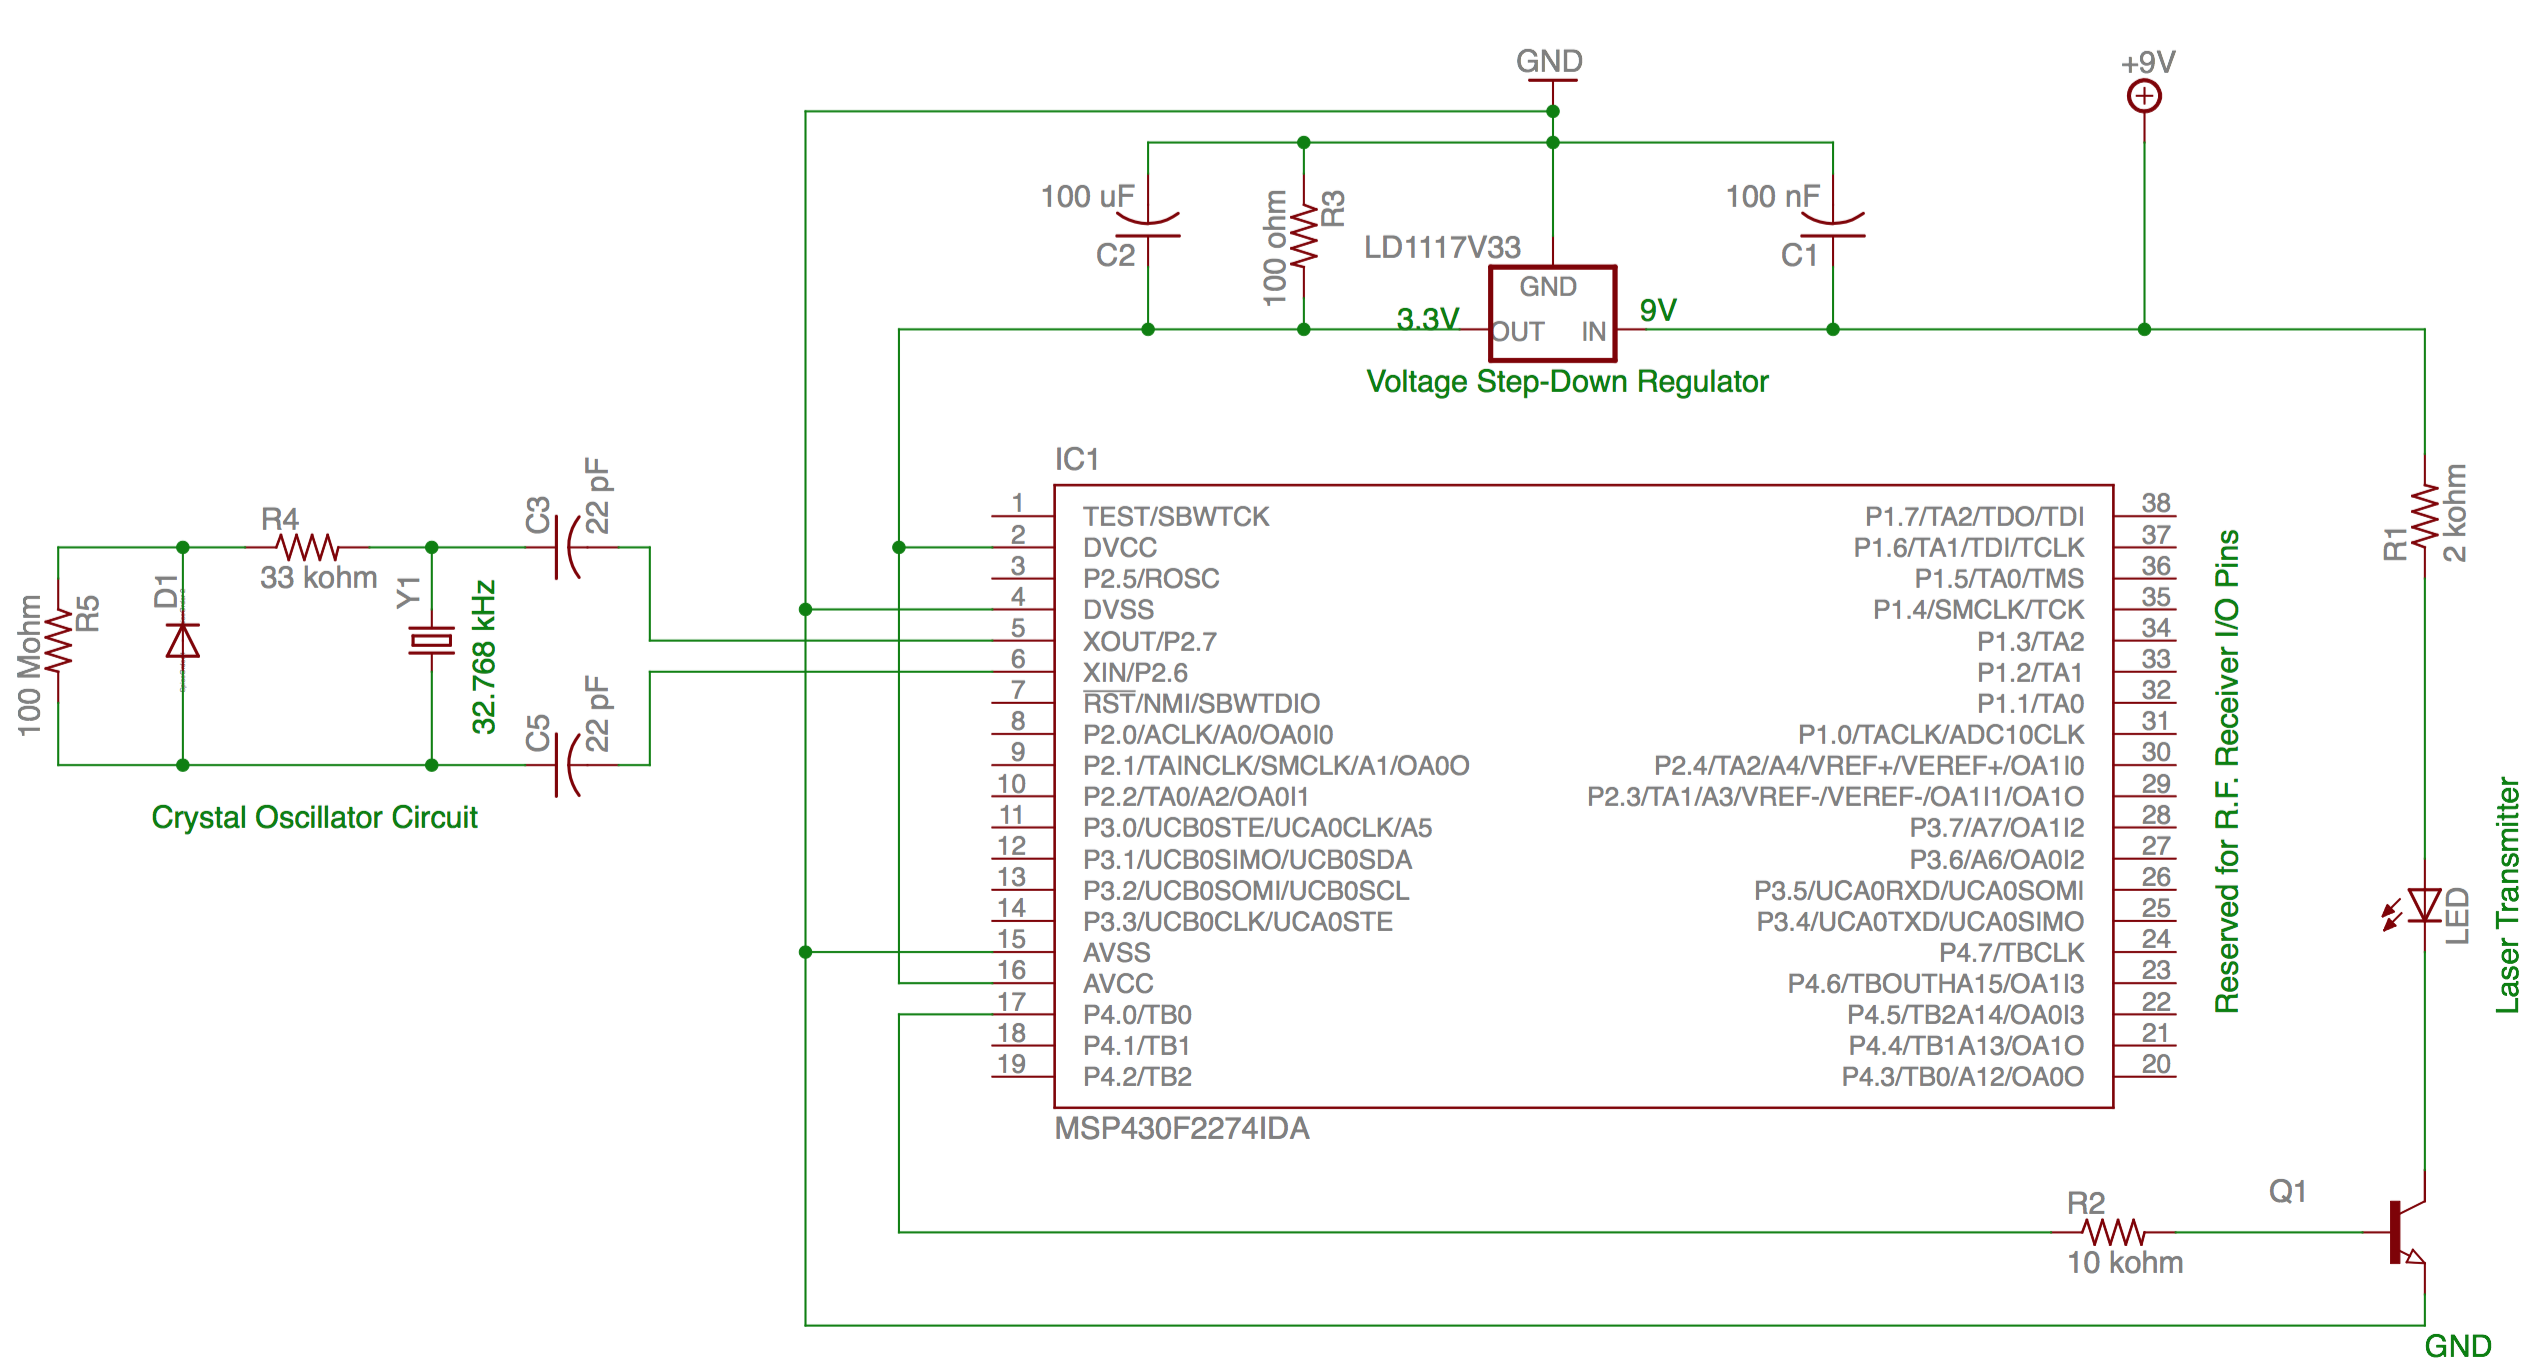
\includegraphics[scale=0.38]{Circuit_Schematic.png}
	\caption{Circuit Schematic of Laser Transmitter\label{fig:circuit-schematic}}
\end{figure}

%SECTION 4 - Plot/Experiment - Noah
\section{Plot}
Figure \ref{fig:nohdplot} depicts the Nominal Ocular Hazard Distance (NOHD) vs the power of the laser diode on a 50\% duty cycle. See \ref{section-safety-ethics} for more details on this calculation and what it means. 
\begin{figure} [H]
	\centering
	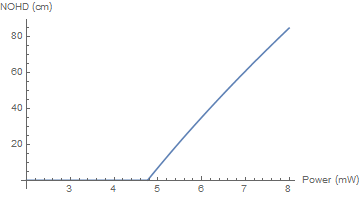
\includegraphics[scale=0.70]{NOHDvsPower.png}
	\caption{NOHD vs Power for Laser Diode\label{fig:nohdplot}}
\end{figure}

%SECTION 5 - Calculations - Both
\section{Calculation}
Please reference Section \ref{section-safety-ethics} for calculations regarding the safety of the laser transmitter. 

%SECTION 6 - Requirements and Verification - Both 
\section{Requirements and Verification}
FILL OUT TOGETHER

%SECTION 7 - Safety - Noah
\section{Safety \& Ethical Considerations} \label{section-safety-ethics}
The proposal requirements would have required a $20mW$ IR laser. However, in the State of Illinois, a 20mW laser is considered a Class 3B laser and must be registered with the Division of Nuclear Safety in the Illinois Emergency Management Agency. This would have required the team to file the correct paperwork and pay a registration fee of \$50. This paperwork would have likely caused delays in receiving parts and construction of this project. A 20 mW laser would have also needed much more pre-caution and safety mitigations than a much less powerful laser.

For the reasons stated above, the team will instead use a $5mW$ visible red laser. $5mW$ visible lasers have a low chance of injuring the eye, as the blinking reflex will save a victim from permanent damage; as opposed to IR lasers which can go unnoticed for several seconds. 

The following is a calculation for the nominal ocular hazard distance (NOHD) of our laser, as defined by the ANSI Standard \cite{ANSI}.

The maximum permissible exposure (MPE), as defined by the ANSI Standard \cite{ANSI} is the highest power or energy density of a light source that is considered safe, i.e. that has a negligible probability for creating damage. This MPE for a pulsing laser is calculated as the minimum of the following three rules:

\begin{enumerate}
	\item Any single pulse in the train must not exceed the MPE for the pulse exposure time.
	\item The exposure from any group of pulses delivered in time T must not exceed the MPE for
	time T, where T is 0.25 seconds (from the blinking reflex), for a visible laser. 
	\item For thermal injury, the exposure for any single pulse within a group of pulses must not
	exceed the single-pulse MPE multiplied by a multiple-pulse correction factor
\end{enumerate}

The laser will pulse at a rate of 40 kHz. Assuming at most a 50\% duty cycle, each pulse will be of max length $1.25*10^{-5} s$. The divergence of the beam is smallest for the longest range; a lower divergence is more restrictive in terms of safety, so this calculation uses $300m$. The divergence of the beam for 300m is 2.79 mrad and the beam waist is approximately $4 mm$. \\

Following the ANSI Standard \cite{ANSI}, the Rule 1 calculation is 

{\large $5*10^{-3}*(\frac{2.79}{1.5})  = 0.0093 \frac{J}{m^2}$ }\\

The Rule 2 calculation is

{\large $\frac{18(.25^{0.75})(\frac{2.79}{1.5})}{.25*40000} = 0.0011837 \frac{J}{m^2}$ }\\

The Rule 3 calculation is

{\large $(.25*40000)^{0.25} * 5*10^{-3}*(\frac{2.79}{1.5}) = 0.093 \frac{J}{m^2}$ }\\

The most restrictive of all the rules is Rule 2, which gives us an MPE of $0.0011837 \frac{J}{m^2}$.

At $5mW$ with a pulse width of $1.25*10^{-5}$, the power of the laser is $6.25*10^{-8} J$. 

The NOHD is defined as

{\LARGE $ \frac{\sqrt{\frac{4 * P}{\pi * MPE}} - 2w}{\theta}$}

Where P is the power of the beam ($6.25*10^{-8} J$) and $w$ is the waist of the beam ($1mm$). This gives an NOHD of 

{\Large$ \frac{\sqrt{\frac{4 * 6.25*10^{-8}}{\pi * 0.0011837}} - 2(0.004)}{0.00279} = 0.0713 m $}
	
The team will avoid eye damage by not working with their eyes inside of 8 cm from the laser. If it is necessary to get this close to the laser, the team will wear eye protection or simply power off the laser. 

\clearpage

\bibliographystyle{IEEE_ECE}
% include the BibTex file here to build reference
\bibliography{Citations}\addcontentsline{toc}{section}{Reference}

\clearpage
\end{spacing}
\end{document}

